\chapter{実装}\label{cha:Implementation}

本章では、本研究で試作したモータ特性表自動生成ツールの実装について説明する。

\section{特性表生成機能}\label{tokuseihyou_seisei}

% モータ特性表自動生成ツールの処理の流れを図\ref{fig:syori}に示す。\\

% \begin{figure}[t]
% 	\centering
% 	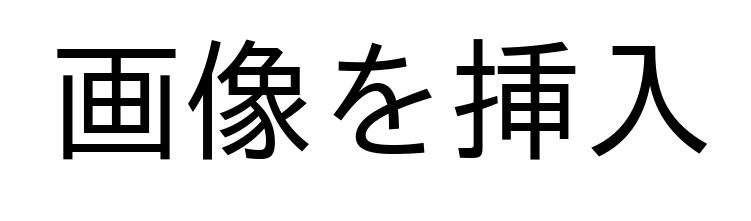
\includegraphics[width=16.5cm,height=10cm]{./Image/sample.png}
% 	\caption{モータ特性表自動生成ツールの処理の流れ}
% 	\label{fig:syori}
%   \end{figure}

特性表生成機能の処理の流れを以下に示す。
\begin{enumerate}
    \item OpenModelicaから出力されたcsvファイルを読み込む
    \item 特性表の各要素を算出するために必要なデータを、csvファイルから取得する
    \item 特性表の各要素を算出する
    \item 特性表を生成する
\end{enumerate}

以下、各処理について具体的に説明する。

\subsection{csvファイルの読み込み}\label{sub:csvfairu}
Pythonで実装するため、Pythonの標準ライブラリのcsvモジュールをインポートし、
csvファイルを読み込む。

\subsection{特性表の各要素を算出するために必要なデータを取得}\label{sub:syutoku_data}
\ref{sub:csvfairu}章で読み込んだcsvファイルから、以下のデータを取得する。

\begin{itemize}
    \item 時間
    \item 電流
    \item 電圧
    \item トルク
    \item 角速度
\end{itemize}

図\ref{fig:simyu_csv}にあるように、OpenModelicaから出力されたcsvファイルの1行目には、
各部品の変数名が記載されている。取得したいデータを持つ変数名を探し、その変数名がある場所の添字を取得する。
そして、各データに対応した配列に、同じ添字の位置にある値を繰り返し処理で格納する方法で値を取得する。

\subsection{特性表の各要素を算出}\label{sub:keisan}
\ref{sub:syutoku_data}章で取得したデータを用いて、\ref{kenkyu_mokuteki}章で挙げた各要素を算出する。

\subsubsection{電圧}\label{sub:sub:dennatu}
シミュレーション時に印加した値を取る。

\subsubsection{始動電流}\label{sub:sub:sidouden}
始動電流とは、モーターの起動時に流れる大きな電流のことである。
モーターが起動した後はモーター自体が発電機にもなり、逆起電力を発生するため、
モーター・コイル部分にかかる電圧が下がり、電流値も下がる。
したがって、電流値の配列の中で一番大きい値を始動電流とする。
% https://www.tsugawa.co.jp/glossary/ 

\subsubsection{停動トルク}\label{sub:sub:teidoutoruku}
停動トルクとは、モーターが出しうる最大トルクで、このトルク以上の負荷がかかれば、モーターは停止する値となる。
したがって、トルク値の配列の中で一番大きい値を停動トルクとする。
% https://www.orientalmotor.co.jp/tech/glossary/ta11/

\subsubsection{最大効率}\label{sub:sub:saidaikouritu}
効率は以下の式で算出することができる。

\[
    \mbox{効率} = \frac{\mbox{出力}}{\mbox{入力}}  * 100 
\]
\[
    \mbox{出力} = \mbox{角速度} * \mbox{トルク} 
\]
\[  
    \mbox{入力} = \mbox{電圧} * \mbox{電力} 
\]

各配列を上記の式に当てはめ、繰り返し処理で効率値の配列を作成する。
最大効率は効率値の配列の中で一番大きい値とする。

% https://www.jp-igarashi.com/product/product_motors/curve.html

\subsubsection{定格トルク}\label{sub:sub:teikakutoruku}
最大効率時のトルクを定格トルクという。
したがって、トルク値の配列の中で、最大効率のある効率値の配列の添字と同じ位置にある値が定格トルクとなる。


% http://www.sagamimicro.co.jp/product/aboutusage.html

\subsubsection{定格回転数}\label{sub:sub:teikakukaiten}
最大効率時の回転数を定格回転数という。
回転数は以下の式で算出することができる。

\[
    \mbox{回転数} = \frac{30 * \mbox{角速度}}{\pi}   
\]

したがって、回転数値の配列の中で、最大効率のある効率値の配列の添字と同じ位置にある値が定格回転数となる。

% https://mathwords.net/kaitensu

\subsubsection{定格電流}\label{sub:sub:teikakuden}
定格電流とは、モータに定格トルクがかかっているときの電流値である。
したがって、電流値の配列の中で、定格トルクのあるトルク値の配列の添字と同じ位置にある値が定格電流となる。

% http://fa-faq.mitsubishielectric.co.jp/faq/show/18504?category_id=1937&site_domain=default

\subsubsection{定格出力}\label{sub:sub:teikakusyutu}
定格出力とは、定格動作点における出力の値である。
定格出力は以下の式で算出することができる。

\[
    \mbox{定格出力} = \mbox{定格回転数} * \mbox{定格トルク} *  \frac{2\pi}{60}
\]

% http://www.nidec-servo.com/jp/digital/pdf/A_technique.pdf

\subsection{特性表を生成}\label{sub:seisei_hyou}
\ref{sub:keisan}で求めた各値を、